% 分子电流和分子磁矩
% 分子|分子电流|分子磁矩|磁场

根据物质电结构学说,任何实物都是由分子、原子组成的,而分子或原子中任何一个电子都不停地同时参与两种运动:一种是环绕原子核的轨道运动,另一种是电子本身的自旋运动.这两种运动都等效于一个电流分布,因而能产生磁效应把分子或原子看作一个整体,分子或原子中各个电子对外界所产生磁效应的总和,可用一个等效的圆电流表示,统称\textbf{分子电流}.这种分子电流具有一定的磁矩,称为\textbf{分子磁矩(molecular magnetic moment)},用符号$\mathbf m_{mole}$表示.

在外磁场$\mathbf B_0$作用下,分子或原子中和每个电子相联系的磁矩都受到磁力矩的作用,由于分子或原子中的电子以一定的角动量作高速转动,这时,每个电子除了保持上述两种运动以外,还要附加电子磁矩以外磁场方向为轴线的转动,称为电子的进动这与力学中所讲的高速旋转着的陀螺,在重力矩的作用下,以重力方向力轴线所作的进动十分相似,如图所示.
\begin{figure}[ht]
\centering
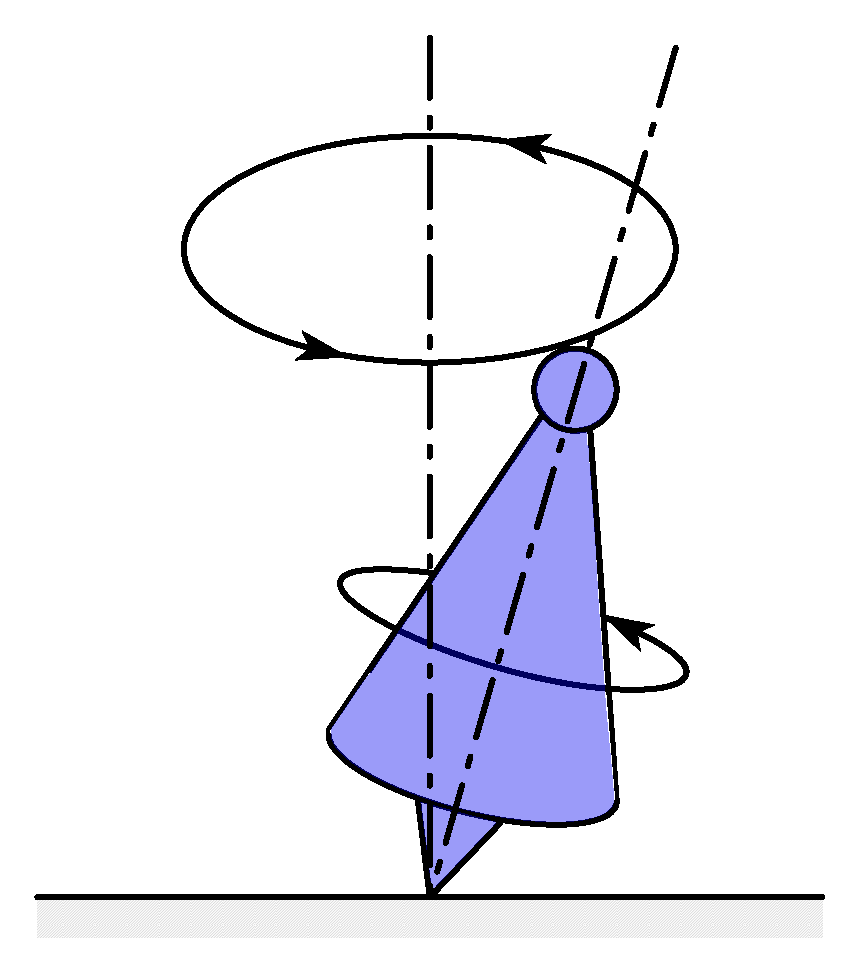
\includegraphics[width=5cm]{./figures/MoMaMo_1.pdf}
\caption{陀螺的进动示意图} \label{MoMaMo_fig1}
\end{figure}
\begin{figure}[ht]
\centering
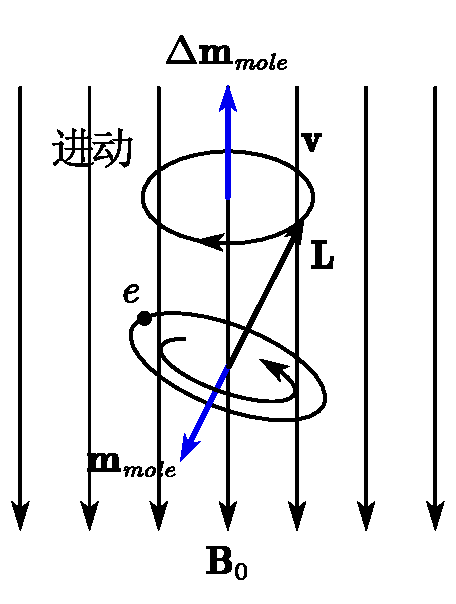
\includegraphics[width=5cm]{./figures/MoMaMo_2.pdf}
\caption{在外磁场中电子的进动和附加磁矩} \label{MoMaMo_fig2}
\end{figure}
\begin{figure}[ht]
\centering
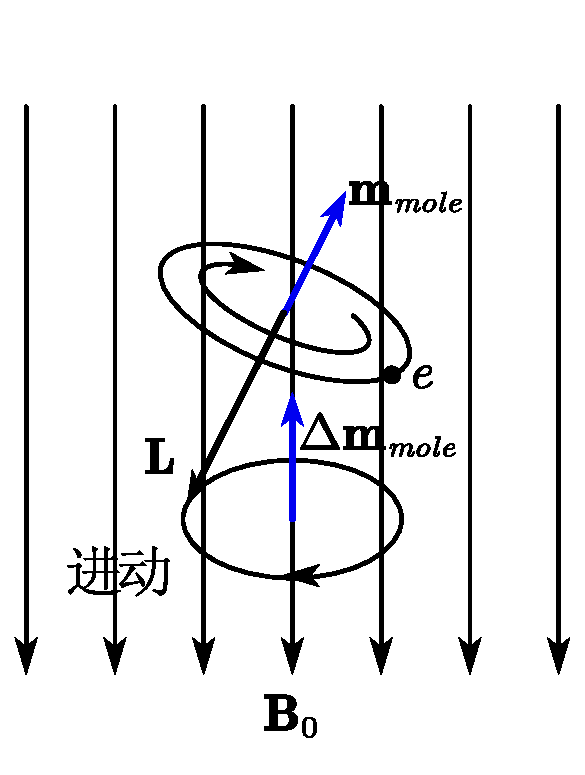
\includegraphics[width=5cm]{./figures/MoMaMo_3.pdf}
\caption{在外磁场中电子的进动和附加磁矩} \label{MoMaMo_fig3}
\end{figure}

我们可以得知,无论电于原来的磁矩与磁场方向之间的夹角是何值,在外磁场$\mathbf B_0$中,电子角动量$\mathbf L$进动的转向总是和$\mathbf B_0$的方向构成右手螺旋关系,如\autoref{MoMaMo_fig2} 和\autoref{MoMaMo_fig3} 所示.电子的进动也相当于一个圆电流.因为电子带负电,这种等效的圆电流的此举的方向永远与$\mathbf B_0$的方向相反,原子或分子中各个电子因进动而产生的磁效应的总和也可用一个等效的分子电流的磁矩来表示,因进动而产生的等效电流的磁矩称为\textbf{附加磁矩},用$\Delta\mathbf m_{mole}$表示.
